\chapter{NPUcore-IMPACT 增量}

在上述基础上,我们继续做了许多努力,让 NPUcore-IMPACT 通过了初赛的所有测试用例,以及初步支持了 EXT4 文件系统。

后文我们会分别详细地介绍这两部分的内容。

\section{初赛测试用例}

我们针对性地对初赛的测试用例进行了调试,将问题归类定位到了如下两点。

然后我们分别对每个问题进行了细致的分析,最终逐个击破,通过了初赛的所有测试用例。

\textbf{1. statx 系统调用}

LoongArch 赛道的初赛测试用例中,mmap 与 munmap 这两个测例涉及到了一个新的系统调用 statx。

\begin{lstlisting}[label={man:statx}, caption={statx 手册}]
NAME
       statx - get file status (extended)

LIBRARY
       Standard C library (libc, -lc)

SYNOPSIS
       #define _GNU_SOURCE          /* See feature_test_macros(7) */
       #include <fcntl.h>           /* Definition of AT_* constants */
       #include <sys/stat.h>

       int statx(int dirfd, const char *restrict pathname, int flags,
                 unsigned int mask, struct statx *restrict statxbuf);

STANDARDS
       Linux.

HISTORY
       Linux 4.11, glibc 2.28.
\end{lstlisting}

如手册 \ref{man:statx} 中所示,这个系统调用涉及了文件信息的获取。

我们为 NPUcore-IMPACT 实现了这个新的系统调用,并与文件系统进行了整合。

\begin{lstlisting}[language={Rust}, caption={statx 系统调用入口}]
let ret = match syscall_id {
    // ...
    SYSCALL_STATX => sys_statx(
        args[0],
        args[1] as *const u8,
        args[2] as u32,
        args[3] as u32,
        args[4] as *mut u8,
    ),
    // ...
};
\end{lstlisting}

\begin{lstlisting}[language={Rust}, caption={statx 系统调用实现}]
pub trait File: DowncastSync {
    // ...
    fn get_statx(&self) -> Statx;
    // ...
}
\end{lstlisting}

随后我们进行了测试,成功通过了 mmap 与 munmap 测试用例。

\textbf{2. 文件描述符分配}

通过对 openat 测试用例进行调试,我们最终发现问题出在操作系统对文件描述符的分配上。

Unix 标准要求操作系统分配文件描述符时,总是分配该进程还未使用的最小的文件描述符;而 NPUcore 回收进程关闭的文件描述符时,使用了一个线性表;操作系统重新分配之前回收的文件描述符时,没有使用表中最小的文件描述符,最终导致出现了问题。

\begin{lstlisting}[language={Rust}, caption={回收文件描述符}]
match self.inner[fd].take() {
    Some(file_descriptor) => {
        self.recycled.push(fd as u8);
        // TODO: maybe replace this with balanced binary tree?
        self.recycled.sort_by(|a, b| b.cmp(a));
        Ok(file_descriptor)
    }
    None => Err(EBADF),
}
\end{lstlisting}

我们选择了在回收文件描述符后进行一次排序来解决这个问题。

这个方案不一定是性能最佳的方案,我们还有以下方案可选:

\begin{enumerate}
    \item 回收时不进行排序,重新分配时使用 $O(n)$ 时间寻找最小的文件描述符;
    \item 使用二叉平衡树替换线性表,从而在 $O(\log n)$ 时间进行回收与重新分配,但也许会带来内存分配的额外开销。
\end{enumerate}

未来此处成为性能瓶颈时,根据性能测试结果选用最优方案会是更好的选择。

\section{文件系统适配}

目前来讲,NPUcore-IMPACT已经完美支持了 fat32 文件系统,但因耦合度较高,目前我们已经对NPUcore羽fat32解耦合,且会支持部分 ext4 文件系统(lwext4)。
而对于适配 fat32 文件系统的具体细节,是我们先前 NPUcore 的增量,不属于我们团队的贡献,因此这里不再赘述,仅在下面给出NPUcore-IMPACT的具体参数。

\subsection{fat32 具体参数}

fat32文件系统是个较为简单的系统,当然,其系统的易移植特性与其简单耐用的特性使其成为了几乎所有系统在初始阶段的第一选择。对于NPUcore-IMPACT,我们可以用一个简单的示意图\ref{fig:fs}来描述他

\begin{figure}[htb]
    \centering
    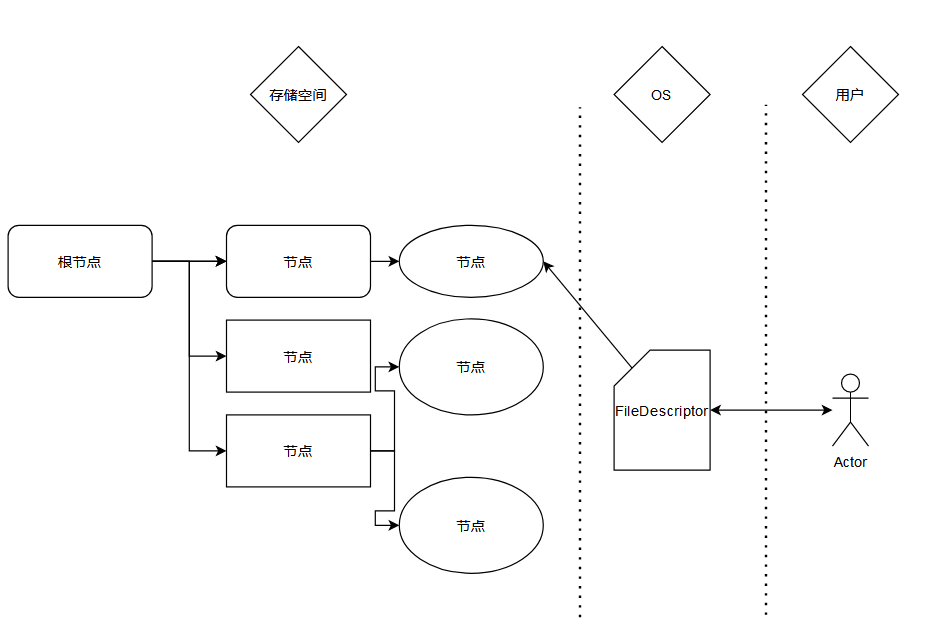
\includegraphics[width=1\linewidth]{figs/dirt.PNG}
    \label{fig:fs}
    \caption{NPUcore-IMPACT的文件系统示意图}
\end{figure}

\subsubsection{FileDescriptor}

如果用简单的描述来简述NPUcore-IMPACT的文件系统,那可以将之理解为一栋楼,我们利用一个描述每个房间的FileDescriptor类的指针来读取一个文件的信息,可以毫不为过的将其理解为我们的文件类型指针, \textbf{FileDescriptor的具体定义如下所示:}

\begin{lstlisting}[language={rust}, label={code:refill}, caption={FileDescriptor}]
    //fs/mod.rs
    #[derive(Clone)]
    pub struct FileDescriptor {
        cloexec: bool,
        nonblock: bool,
        pub file: Arc<dyn File>,
    }
\end{lstlisting}

\subsubsection{文件树结构}

以下是我们定义文件树节点的结构体:

\begin{lstlisting}[language={rust}, label={code:refill}, caption={FileDescriptor}]
    pub struct DirectoryTreeNode {
        /// If this is a directory
        /// 1. cwd
        /// 2. mount point
        /// 3. root node
        /// If this is a file
        /// 1. executed by some processes
        /// This parameter will add 1 when opening
        spe_usage: Mutex<usize>,
        name: String,
        filesystem: Arc<FileSystem>,
        file: Arc<dyn File>,
        selfptr: Mutex<Weak<Self>>,
        father: Mutex<Weak<Self>>,
        children: RwLock<Option<BTreeMap<String, Arc<Self>>>>,
    }
\end{lstlisting}

在通过文件树寻找制定文件的过程中,首先会判断文件的路径前缀是否在路径缓存
中,这样使大量文件操作效率更高,同时 NPUcore 也对一些默认的路径进行了路径的
转化,这部分将于后续5.4中详细说明。

\subsection{NPUcore-IMPACT BitFlags一览}

我们遵循原版POSIX的flag编码,源码如下:
\begin{lstlisting}[language={rust}, label={code:refill}, caption={FileDescriptor}]
    bitflags! {
        pub struct OpenFlags: u32 {
            const O_RDONLY      =   0o0;
            const O_WRONLY      =   0o1;
            const O_RDWR        =   0o2;

            const O_CREAT       =   0o100;
            const O_EXCL        =   0o200;
            const O_NOCTTY      =   0o400;
            const O_TRUNC       =   0o1000;

            const O_APPEND      =   0o2000;
            const O_NONBLOCK    =   0o4000;
            const O_DSYNC       =   0o10000;
            const O_SYNC        =   0o4010000;
            const O_RSYNC       =   0o4010000;
            const O_DIRECTORY   =   0o200000;
            const O_NOFOLLOW    =   0o400000;
            const O_CLOEXEC     =   0o2000000;
            const O_ASYNC       =   0o20000;
            const O_DIRECT      =   0o40000;
            const O_LARGEFILE   =   0o100000;
            const O_NOATIME     =   0o1000000;
            const O_PATH        =   0o10000000;
            const O_TMPFILE     =   0o20200000;
        }
    }

    bitflags! {
        pub struct SeekWhence: u32 {
            const SEEK_SET  =   0; /* set to offset bytes.  */
            const SEEK_CUR  =   1; /* set to its current location plus offset bytes.  */
            const SEEK_END  =   2; /* set to the size of the file plus offset bytes.  */
        }
    }

    bitflags! {
        pub struct StatMode: u32 {
            ///bit mask for the file type bit field
            const S_IFMT    =   0o170000;
            ///socket
            const S_IFSOCK  =   0o140000;
            ///symbolic link
            const S_IFLNK   =   0o120000;
            ///regular file
            const S_IFREG   =   0o100000;
            ///block device
            const S_IFBLK   =   0o060000;
            ///directory
            const S_IFDIR   =   0o040000;
            ///character device
            const S_IFCHR   =   0o020000;
            ///FIFO
            const S_IFIFO   =   0o010000;

            ///set-user-ID bit (see execve(2))
            const S_ISUID   =   0o4000;
            ///set-group-ID bit (see below)
            const S_ISGID   =   0o2000;
            ///sticky bit (see below)
            const S_ISVTX   =   0o1000;

            ///owner has read, write, and execute permission
            const S_IRWXU   =   0o0700;
            ///owner has read permission
            const S_IRUSR   =   0o0400;
            ///owner has write permission
            const S_IWUSR   =   0o0200;
            ///owner has execute permission
            const S_IXUSR   =   0o0100;

            ///group has read, write, and execute permission
            const S_IRWXG   =   0o0070;
            ///group has read permission
            const S_IRGRP   =   0o0040;
            ///group has write permission
            const S_IWGRP   =   0o0020;
            ///group has execute permission
            const S_IXGRP   =   0o0010;

            ///others (not in group) have read, write,and execute permission
            const S_IRWXO   =   0o0007;
            ///others have read permission
            const S_IROTH   =   0o0004;
            ///others have write permission
            const S_IWOTH   =   0o0002;
            ///others have execute permission
            const S_IXOTH   =   0o0001;
        }
    }
\end{lstlisting}

